\documentclass[main.tex]{subfiles}
\begin{document}


\chapter{Prototyp}
Um heraus zu finden welche der OSRE am performantesten ist, wurden drei Prototypen erstellt. Mit diesen soll erforscht werden, wie sich eine Applikation beim Einsatz der verschiedenen ORSE verhaltet. Es wurde darauf geachtet das der Prototyp nur genau die Komponenten besitzt die es für die Aufgabe benötigt.  

Jeder Prototyp ist in zweiteilig , die Prototypen besitzen die gleiche REST-Schnittstelle welche die Anfragen entgegen nimmt. Die REST-Schnittstelle leitet diese Anfrage  an die entsprechende Implementationen weiter. Dort werden diese Anfragen in konkrete PDFs umgesetzt. Im folgenden werden die Grundlegenden Aspekten der Implementationen näher betrachtet. 


\section{Schnittstelle}


Die Schnittstelle wurde so implementiert, das eine \acrshort{http}-POST Anfrage entgegengenommen werden kann. Den Request-Body wird dem Interface '\texttt{PdfEngine}' weitergegeben. Dieses Interface wurde mithilfe der Spring-Annotation @Autowired injected. Damit besteht eine lose Koppelung der \acrshort{pdf}-Implementation und der Schnittstelle gegen aussen. Dank dieser Aufstellung kann nun einfach eine beliebige Implementation aufgerufen werden.

Die \acrshort{rest}-Schnittstelle bietet die drei PDF-Szenarien über die Endpunkte \texttt{/scenario1}, \texttt{/scenario2} und \texttt{/scenario3} an.   

\begin{lstlisting}[language=Java]
@RestController("/")
public class PdfServiceController {

	@Autowired
	private PdfEngine engine;

	@RequestMapping(method = RequestMethod.POST, path = "scenario1")
	public @ResponseBody PdfResponse scenario1(@RequestBody PdfRequestScenario1 req) {
		return engine.createPdfSzenario1(req);
	}
     ...
}
\end{lstlisting}

\subsection{Requests}
Die Endpunkte werden mit den folgenden \gls{post}-Bodys angesprochen. 


\subsubsection{Szenario 1}
Das \acrlong{json} für das erste Szenario bildet das Modell für eine Aktivität ab. Diese soll einen Titel und eine Zeitangabe besitzen wann diese stattfindet. Es wurden verschiedene Informationen hinterlegt die für eine Freizeitbeschäftigung interessant wären, wie wer organisiert und welche Freunde oder Helfer eingeladen werden, sowie wo es stattfinden soll.  
\begin{lstlisting}[language=json]
{"data": [
      {
      "title":          "Sommer-Fest",
      "datumVon":       "12.02.2017 16:00",
      "datumBis":       "12.02.2017 23:00",
      "description":    "Bringt Essen und gute Laune mit",
      "place":          "Musterstrasse 12\n888 Musterstadt\nSchweiz",
      "incharge":       "Denis Bittante",
      "helper":         "Lars Hauser, Max Muster",
      "author":         "Denis Bittante"
   }, ...
]}


\end{lstlisting}


\subsubsection{Szenario 2}
Szenario 2 ist sozusagen eine Zusammenfassung oder Programm der interessanten Aktivitäten an einem Tag anstehen werden. Die Daten fassen die Eckdaten einer Aktivität zusammen wie der Organisator und die Zeitangaben. Es gibt keine Details aber eine Möglichkeit eine Fussnote zu versehen die nach jedem Tag erscheinen soll. 
\begin{lstlisting}[language=json]
{"group": [
      {
      "title":  "21.2.12 Vortraege fuer diesen Tag",
      "entries":[ {
            "time":         "19:00",
            "title":        "Ein Titel",
            "person":       "D.Bittante",
            "isSubtitle":   false
         },  ...
      ],
      "footer": "Special Information as Footnote"
   }, ...
      ]}


\end{lstlisting}


\subsubsection{Szenario 3}

Im dritten Szenario wurde entscheiden eine Kontaktliste darzustellen, damit die Helfer und Freunde auch ausgedruckt werden können. In Hinblick festzustellen wie die \acrlong{osre} mit Bilder und Tabellen umgeben könenn wurde hier entschieden die Personendaten wie Vorname, Familienname und Adress- und Kontaktdaten zu hinterlegen aber auch die Information des Geschlechts dabei steht 'm' für männlich (male) und 'f' für female. Die Gender-Information soll dann auf der Kontaktliste als Gender-Symbol dargestellt werden. 

\begin{lstlisting}[language=json]
{"contacts": [
      {
      "gender":     "m",
      "name":       "Mustername",
      "firstname":  "Max",
      "address":    "Musterstrasse 12",
      "zip":        "9000",
      "place":      "Ort",
      "tel":        "+41 55 555 55 55",
      "mob":        "+41 55 555 55 55",
      "birthday":   "2.2.1988",
      "note":       "schlaue Notiz fuer diese Person",
      "email":      "max.muster2000@gmx.ch"
   }, ...
]}


\end{lstlisting}

\begin{reference}{JSON Request}
 Vollständige Request können unter \url{https://github.com/denisbittante/dinf/tree/master/loadtest/testdata} gefunden werden.
\end{reference}
 


\subsection{Responses}
Die Responses der REST-Schnittstelle wurden einfach gehalten, daher wird die OSRE und das Szenario angegeben und im Feld \texttt{status} ob die Verarbeitung korrekt abgeschlossen wurde. Das generierte PDF ist als base64 encodiert und als Feld \texttt{file} in der Response zu finden. 
\begin{lstlisting}[language=json]
{
   "name": "ApachePdfBox",
   "description": "Szenario 1",
   "file": "JVBERi0xLjQKJfb ... hyZWYKMTc2NAolJUVPRgo=",
   "status": "ok"
}

\end{lstlisting}




\section{PDF Generierung}

Beim Injecten des Interfaces PDFEngine werden je nach Build eines der drei Implementationen instanziert (siehe Abbildung \ref{figure:pdfEngineImpl}). Jeder dieser Klassen hat alle drei Szenarien zu implementieren.  


\begin{figure}[h]
 
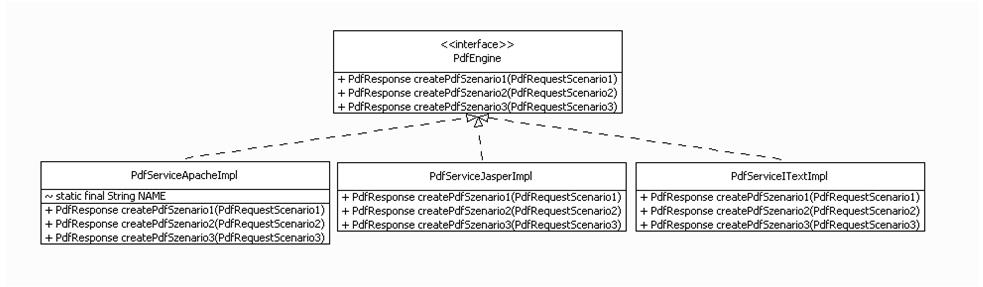
\includegraphics[width=\textwidth ]{pic/uml/PdfEngineImplemntierung.jpg}
 \caption{UML PDFEngine Implementierungen}
 \label{figure:pdfEngineImpl}
\end{figure}

Die einzelne Szenarien wurden ebenfalls als Interfaces deklariert damit jedes dieser Szenarios nicht anders oder nur teilweise implementiert wird. Als Basis-Klasse wurde die AbstractScenario-Klasse implementiert, diese regelt den Aufbau und wie die Temporären Files auf dem System abgelegt werden und diese wieder abgeräumt werden. Diese abstrakte Klasse übernimmt ebenfalls den Aufbau und und das Handling des PdfRequest als Business-Model. Dieses Model steht jeder Implementation über die Methode getModel zur Verfügung.   

\begin{figure}[h]
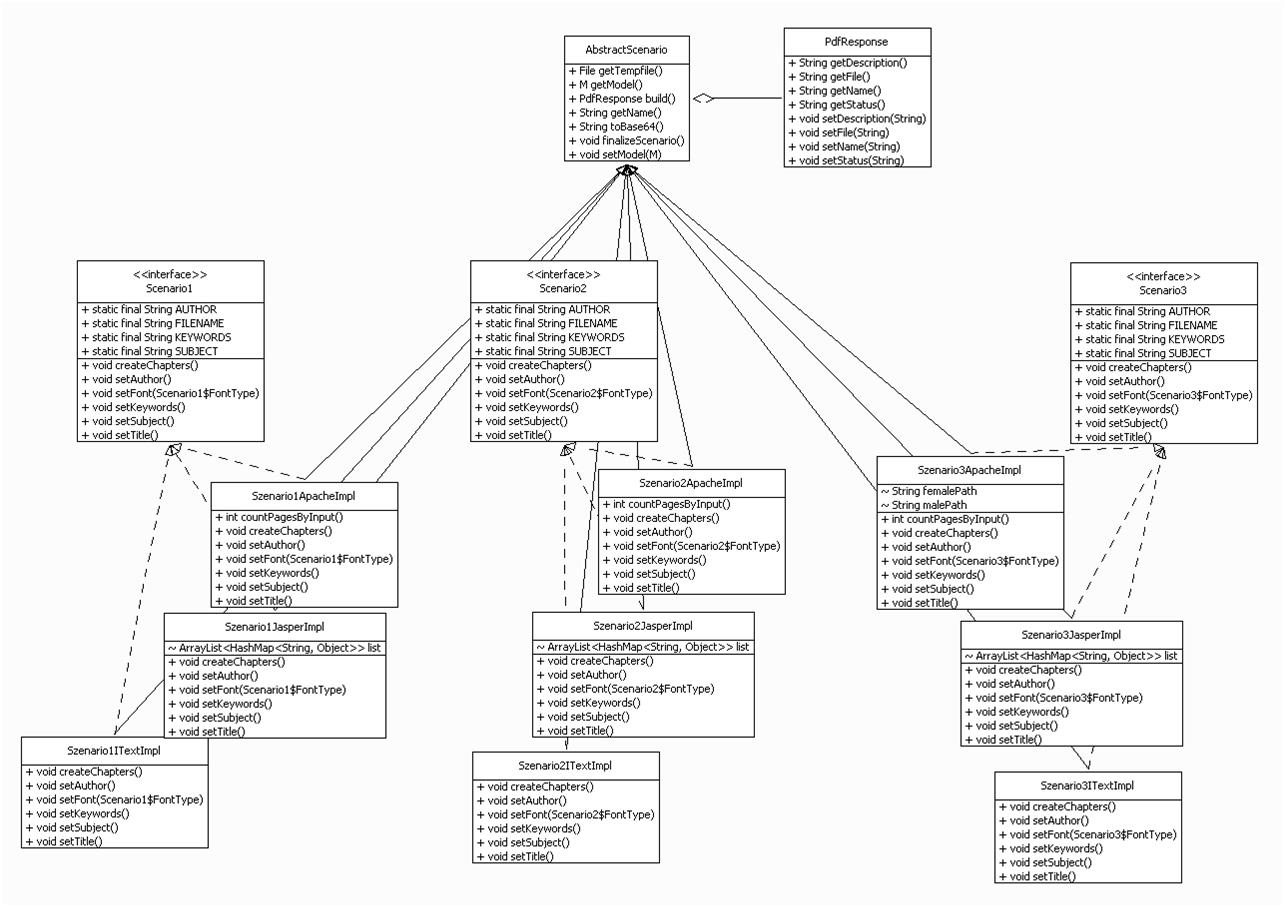
\includegraphics[width=\textwidth ]{pic/uml/SzenarioImplementation.jpg}
 \caption{UML Szenario Implementierungen}
 \label{figure:szenImpl}
\end{figure}



\subsection{Build / Deployment}

Die einzelnen Jars mit den gewünschten implementation können mittels Maven gebildet werden dazu wurden für jedes Produkt ein Profil eingerichtet. Dafür muss das Projekt vollständig gebildet werden, damit die einzelnen Implementationen als Archiv im Maven Repository erreichbar sind und anschliessend kann der REST-Service gebildetet und gestartet werden.  

\begin{lstlisting}[language=command.com]


REM Bildet alle Maven Module 
cd ../dinf/app/ 
mvn clean install 

REM  Bildet den RestService mit gewuenschter OSRE Implementation     
cd ../dinf/app/rest-springboot/

mvn clean install -Pitext
REM (oder)
mvn clean install -Pjasper
REM (oder)
mvn clean install -Ppdfbox
\end{lstlisting}


Das generierte Jar kann über den heroku Komando ebenfalls über die Console deployed werden. Das der Stand des gewünschten Dyno meist nicht bekannt ist wurde nach dem Deployment auch den Dyno neu gestartet. 

\begin{lstlisting}[language=command.com]

REM Deployed hier denn service mit der pdfbox implementation auf den Dyno 'dinf-app'
heroku deploy:jar  target\rest-service-pdfbox.jar --app dinf-app

REM Startet den Dyno namens 'dinf-app' erneut
heroku restart --app dinf-app



\end{lstlisting}

\subsection{Technische Details}

Folgende technischen Eckdaten sind in diesem Experiment  von Vorteil um ähnliche Performance-Ergebnisse erzielen zu könenn. 

Es wurden folgene Versionen genutzt: 


\begin{table}[!hb]
\label{softversion}
\begin{tabular}{ll}
Software          & Version   \\ \hline
Java        &      jdk 1.8.0.112      \\
Spring Boot &         1.5.8.RELEASE        \\

iText        &        7.1.0  \\
Apache PDFBox - Core &  2.0.1 \\
Apache PDFBox - fontbox & 2.0.0 \\
Apache PDFBox - jempbox & 1.8.11 \\
Apache PDFBox - xmpbox & 2.0.0 \\
Apache PDFBox - preflight & 2.0.0 \\
Apache PDFBox - pdfbox-tools & 2.0.0 \\
JasperReport & 6.4.3 \\
JasperReport - fonts & 4.0.0 \\
Maven   &  3.3.9 \\
 & \\

Heroku (PaaS)    & \\ \hline
Region & USA \\
Stack & heroku-16 \\
Buildpacks & heroku/jvm \\
Dyno Type & Standard-2X \\
RAM & 1GB \\
Anzahl Dyno & 1 \\


\end{tabular}
\caption{Technische Angaben}
\end{table}




\end{document}
